\documentclass[a4paper,12pt]{article}
\usepackage{geometry}
 \geometry{
 a4paper,
 total={170mm,257mm},
 left=20mm,
 top=20mm,
 }
\usepackage{adjustbox}
\usepackage[polish]{babel}
\usepackage{polski}
\usepackage{multirow}
\usepackage{makecell}
\usepackage{boldline}
\usepackage[T1]{fontenc} 
\usepackage{listings}
\usepackage{color}
\usepackage{biblatex}
\usepackage{csquotes}
\usepackage{indentfirst}
\usepackage{subfig}
\addbibresource{gitkraken.bib}

\lstset{literate={ą}{{\k{a}}}1 {ł}{{\l{}}}1 {ń}{{\'n}}1 {ę}{{\k{e}}}1 {ś}{{\'s}}1 {ż}{{\.z}}1 {ó}{{\'o}}1 {ź}{{\'z}}1 {Ą}{{\k{A}}}1 {Ł}{{\L{}}}1 {Ń}{{\'N}}1 {Ę}{{\k{E}}}1 {Ś}{{\'S}}1 {Ż}{{\.Z}}1 {Ó}{{\'O}}1 {Ź}{{\'Z}}1 {Ć}{{\'C}}1 {ć}{{\'c}}1 }

\title{}
\author{Jakub Kraus}
\date{23.01.2024}
\renewcommand\theadalign{tl}
\begin{document}
\renewcommand{\arraystretch}{2}
\begin{table}[ht]
    \centering
    \begin{adjustbox}{width=1\textwidth,center=\textwidth}
        \begin{tabular}{V{4}lV{4}c|c|c|c|c|c V{4}}
            \hlineB{4}
            \multicolumn{2}{V{4}lV{4}}{}                                         & \multicolumn{5}{lV{4}}{\textbf{Wydział Nauk Ścisłych i Technicznych}}                                                                                                                                   \\
            \cline{3-7}
            \multicolumn{2}{V{4}cV{4}}{\textbf{Uniwersytet Śląski w Katowicach}} & \multicolumn{5}{lV{4}}{\textbf{Instytut Fizyki}}                                                                                                                                                        \\
            \cline{3-7}
            \multicolumn{2}{V{4}lV{4}}{}                                         & Rok                                                                   & \textbf{III}                                          & Semestr                            & \multicolumn{2}{cV{4}}{\textbf{V}} \\
            \hlineB{4}
            Kierunek                                                             & \multicolumn{6}{cV{4}}{Informatyka stosowana}                                                                                                                                                           \\
            \hline
            Przedmiot                                                            & \multicolumn{6}{cV{4}}{\textbf{SiNWO - laboratorium}}                                                                                                                                                   \\
            \hlineB{4}
            Prowadzący                                                           & \multicolumn{6}{cV{4}}{dr Wojciech Gurdziel}                                                                                                                                                            \\
            \hline
            Tytuł ćwiczenia                                                      & \multicolumn{4}{c|}{\textbf{Git - aplikacje}}                         &
            \multirow{2}{*}{Nr ćwiczenia}                                        & \multirow{2}{*}{\textbf{II}}                                                                                                                                                                            \\
            \cline{1-5}
            \thead{Sprawozdanie wykonał:                                                                                                                                                                                                                                                   \\ (Imię i Nazwisko)} &
            \multicolumn{4}{c|}{\textbf{Jakub Kraus}}                            &                                                                       &                                                                                                                                 \\
            \hlineB{3}
            Data wykonania ćwiczenia                                             & \textbf{23.01.2024}                                                   & \multicolumn{2}{V{4}lV{4}}{Data oddania sprawozdania} & \multicolumn{3}{cV{4}}{01.02.2024}                                      \\
            \hlineB{4}
        \end{tabular}
    \end{adjustbox}
\end{table}
\newpage
\tableofcontents

\newpage
\clearpage

\listoffigures
\lstlistoflistings
\newpage



\section{Cel ćwiczenia}
Celem ćwiczenia było zapoznanie się z aplikacjami do obsługi systemu kontroli wersji Git.
\section{Przebieg ćwiczenia}
Do wykonania ćwiczenia postanowiłem użyć narzędzie GitKraken oraz system operacyjny Windows 11.
\subsection{Blame}
\begin{lstlisting}[caption={Blame w terminalu},captionpos=b]
    $ git blame 344120
\end{lstlisting}
\begin{figure}[ht]
    \centering
    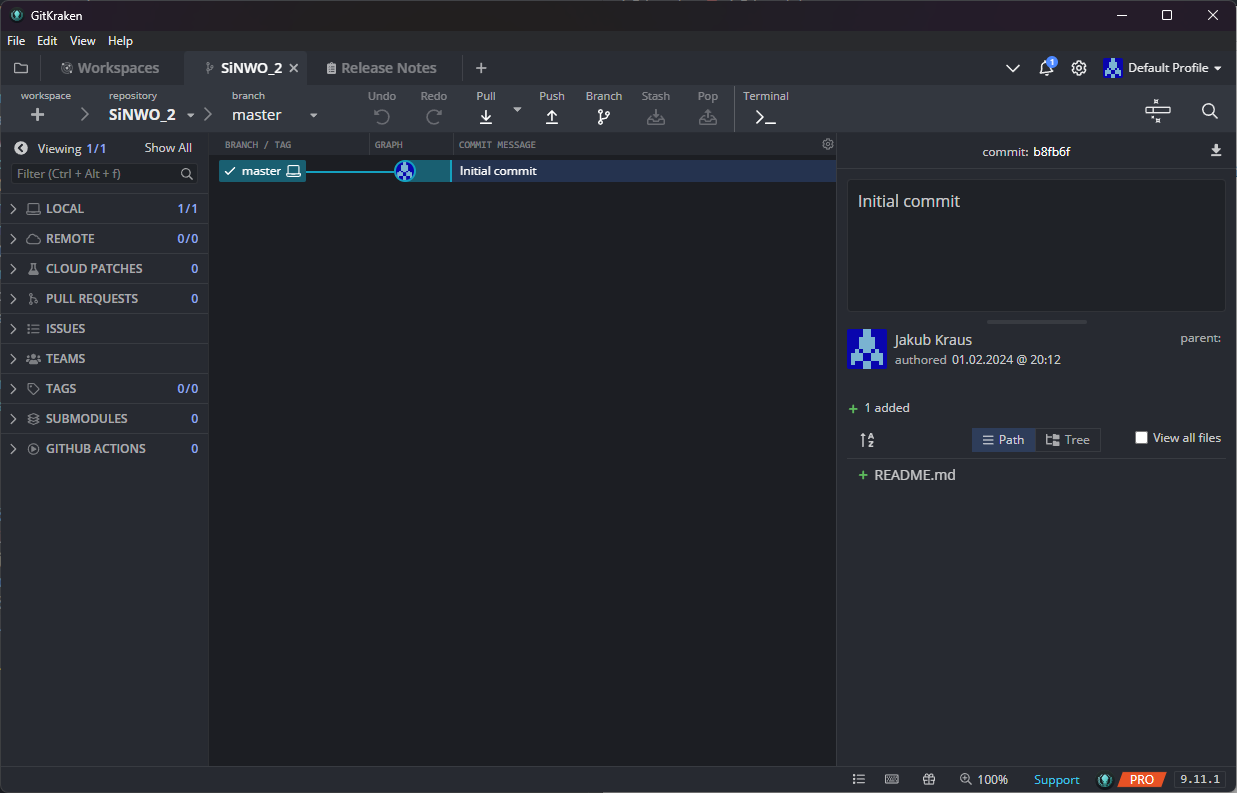
\includegraphics[width=1\textwidth]{images/blame.png}
    \caption{git blame w GitKraken}
\end{figure}

\newpage
\clearpage

\subsection{Checkout}
\begin{lstlisting}[caption={Checkout w terminalu},captionpos=b]
    $ git checkout test_branch
\end{lstlisting}
\begin{figure}[ht]
    \centering
    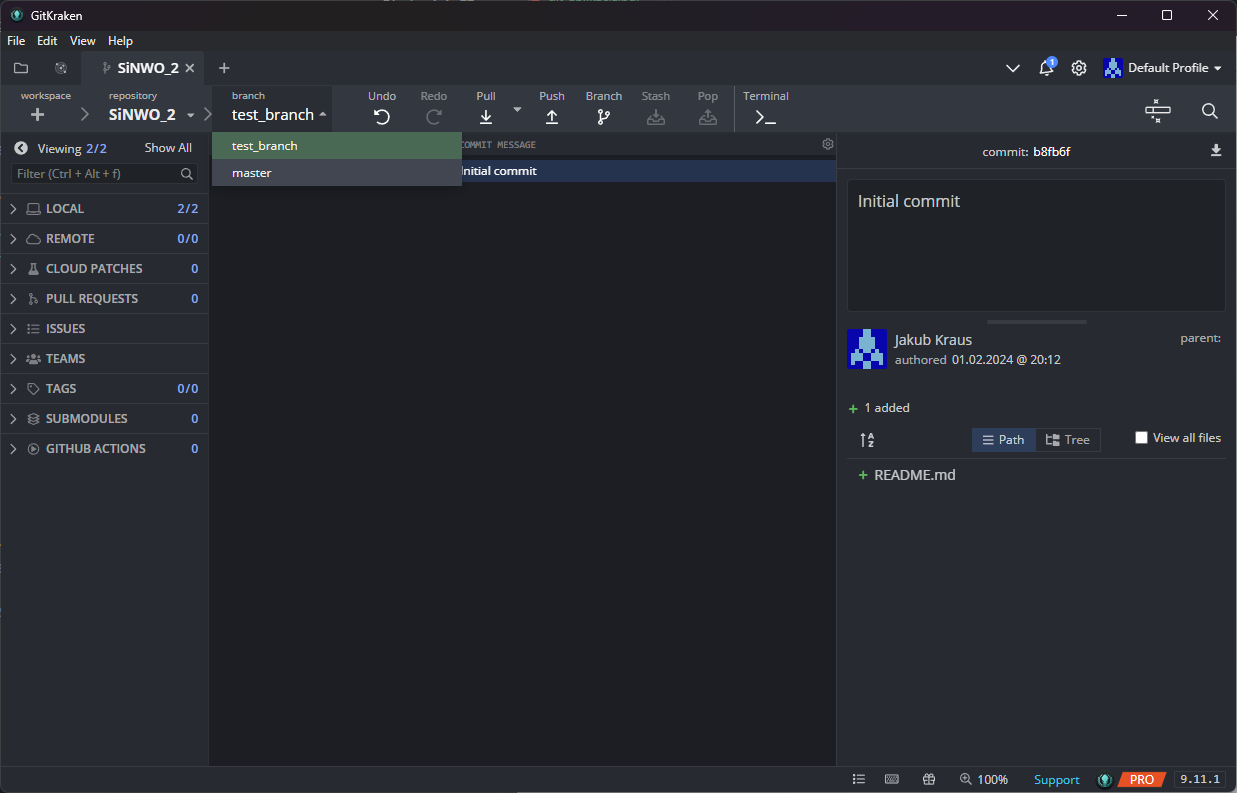
\includegraphics[width=0.7\textwidth]{images/checkout.png}
    \caption{git checkout w GitKraken}
\end{figure}
\subsection{Merge}
\begin{lstlisting}[caption={Scalanie w terminalu},captionpos=b]
    $ git merge test_branch
\end{lstlisting}
\begin{figure}[ht]
    \centering
    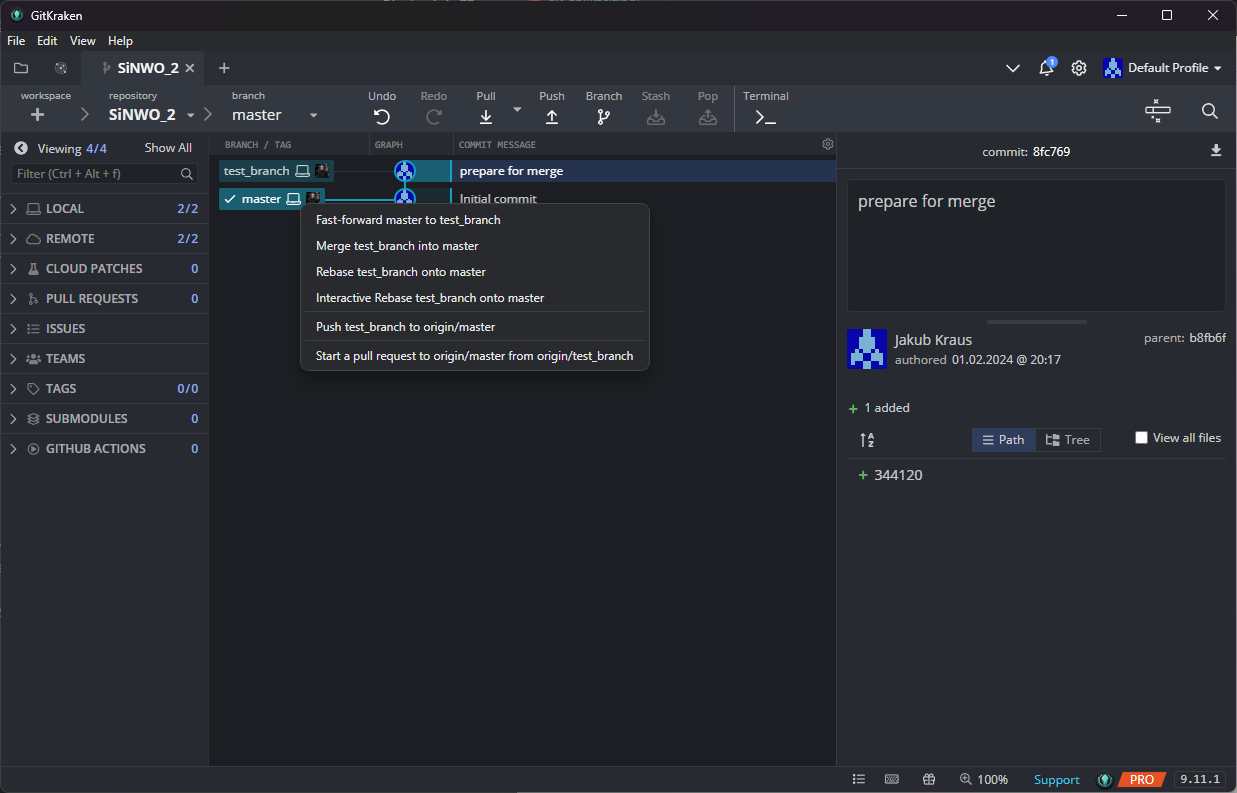
\includegraphics[width=0.8\textwidth]{images/merge.png}
    \caption{git merge w GitKraken}
\end{figure}

\newpage
\clearpage

\subsection{Konflikt scalania}
\begin{lstlisting}[caption={Konflikt scalania w terminalu},captionpos=b]
    $ git merge test_branch
    Auto-merging 344120
    CONFLICT (content): Merge conflict in merge.txt
    Automatic merge failed; fix conflicts and then commit the result.
\end{lstlisting}
\begin{figure}[ht]
    \centering
    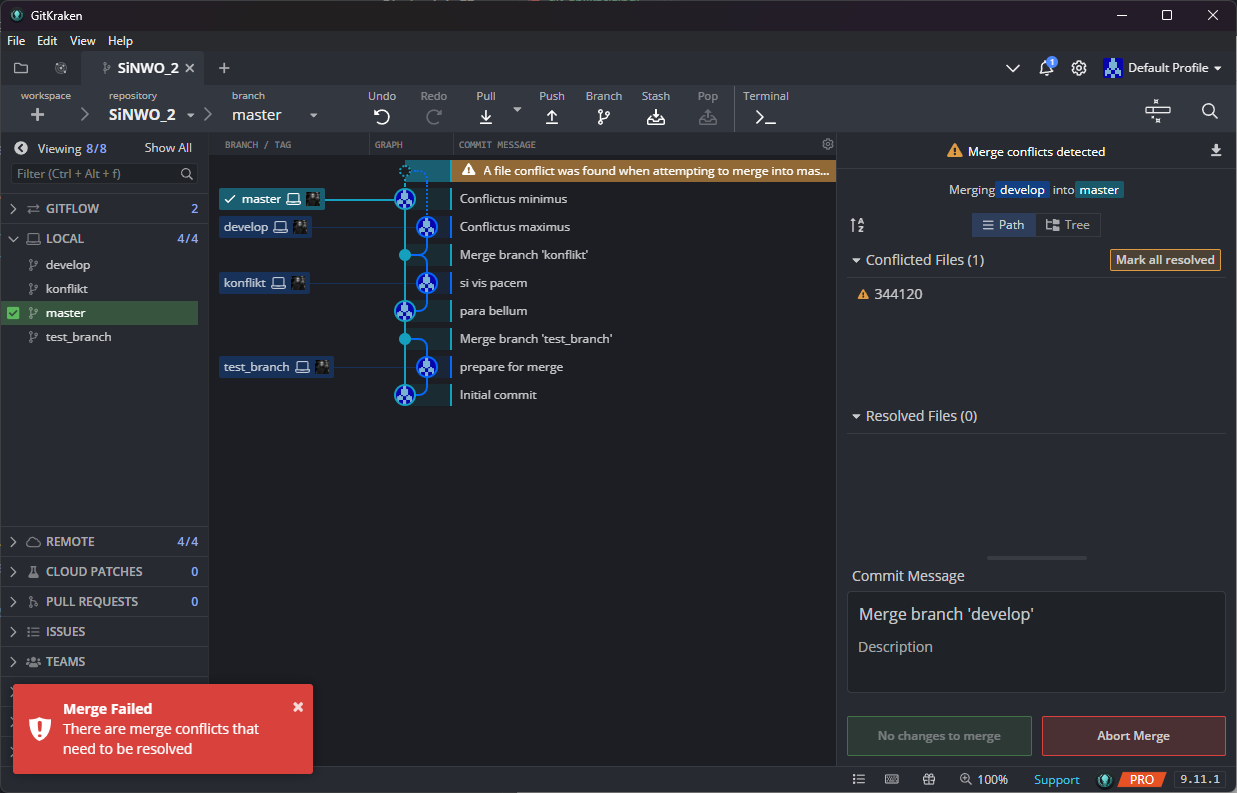
\includegraphics[width=0.6\textwidth]{images/conflict.png}
    \caption{Konflikt scalania w GitKraken}
\end{figure}



\subsection{Merge tool}
Git mergetool można w skonfigurować, aby używał wybranego przez nas narzędzia do rozwiązywania konfliktów. W moim przypadku jest to vimdiff.
\begin{lstlisting}[caption={Komenda mergetool w terminalu},captionpos=b]
    $ git config --global merge.tool vimdiff
    $ git mergetool
\end{lstlisting}
\begin{figure}[ht]
    \centering
    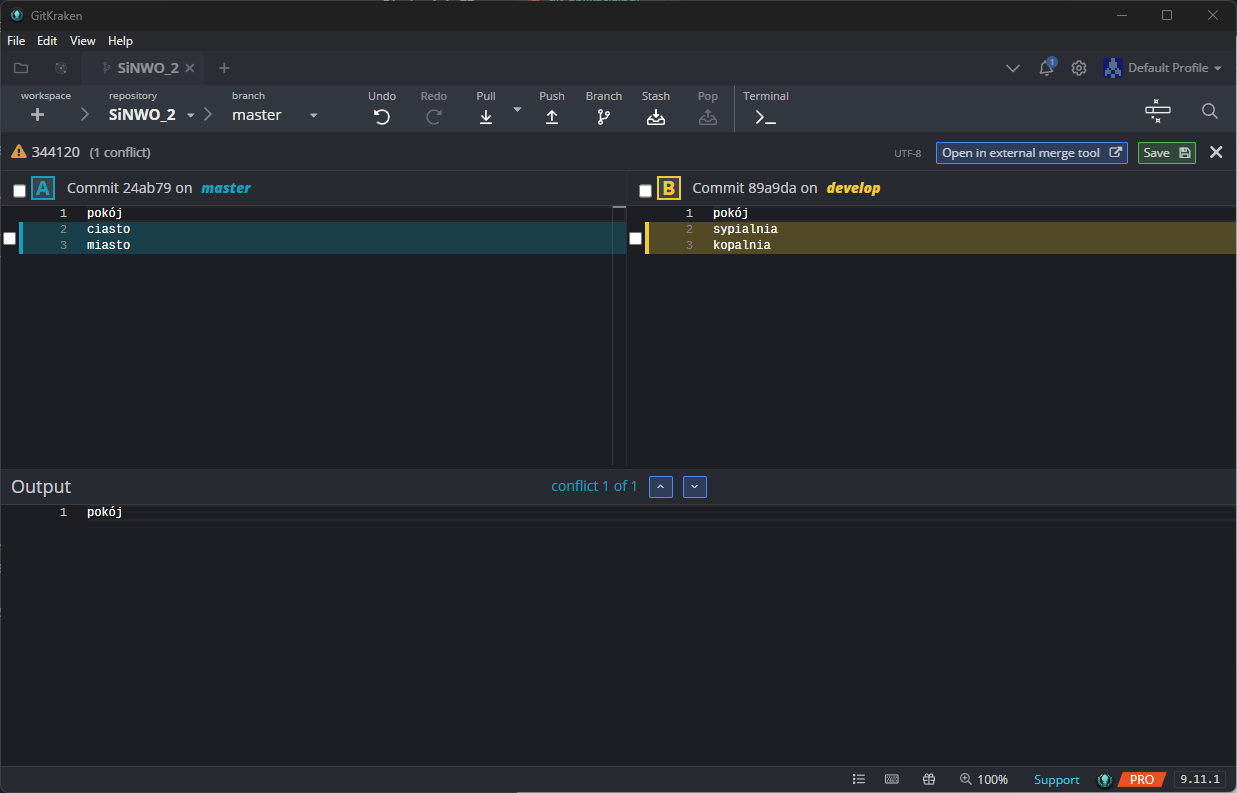
\includegraphics[width=0.60\textwidth]{images/merge-tool.png}
    \caption{Mergetool w GitKraken}
\end{figure}
\subsection{diff --word-diff}
Word diff jest domyślnie włączony w GitKrakenie. W terminalu można go włączyć za pomocą polecenia:
\begin{lstlisting}[caption={diff --word-diff w terminalu},captionpos=b]
    $ git diff --word-diff
\end{lstlisting}
\begin{figure}[ht]
    \centering
    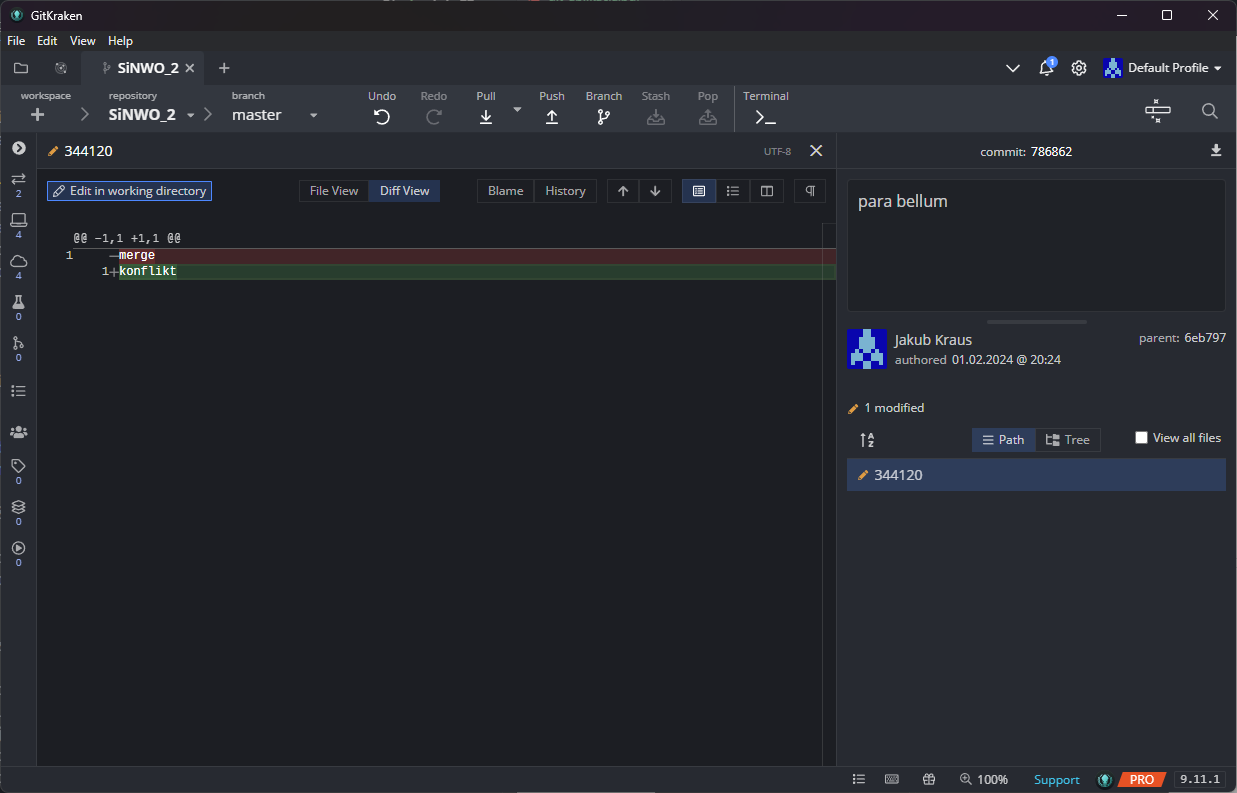
\includegraphics[width=0.8\textwidth]{images/diff.png}
    \caption{diff-word-diff w GitKraken}
\end{figure}
\subsection{log --graph --oneline}
\begin{lstlisting}[caption={log --graph --oneline w terminalu},captionpos=b]
    $ git log --graph --oneline
\end{lstlisting}
\begin{figure}[ht]
    \centering
    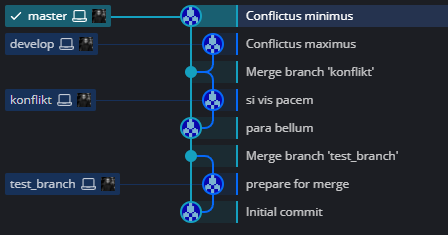
\includegraphics[width=0.78\textwidth]{images/log.png}
    \caption{log --graph --oneline w GitKraken}
\end{figure}

\newpage
\clearpage

\subsection{Aliasy}
Nie udało mi się znaleźć w GitKrakenie opcji do tworzenia aliasów.

\begin{lstlisting}[caption={Przykładowy alias w terminalu},captionpos=b]
    $ git config --global alias.lg "log --graph --oneline"
\end{lstlisting}
\subsection{Klonowanie z SSH}
Aby móc sklonować repozytorium z SSH należy najpierw wygenerować klucz SSH, a następnie dodać go do swojego konta na GitHubie. W przeciwieństwie do konfiguracji SSH w terminalu, w GitKrakenie nie trzeba robić nic, oprócz wygenerowania klucza i dodania go do konta na GitHubie. Po zrobieniu tego, można już klonować repozytorium z SSH.
\begin{lstlisting}[caption={Klonowanie z SSH w terminalu},captionpos=b]
    $ git clone git@github.com:alkatraz445/SiNWO_2.git
\end{lstlisting}

\begin{figure}[ht]
    \centering
    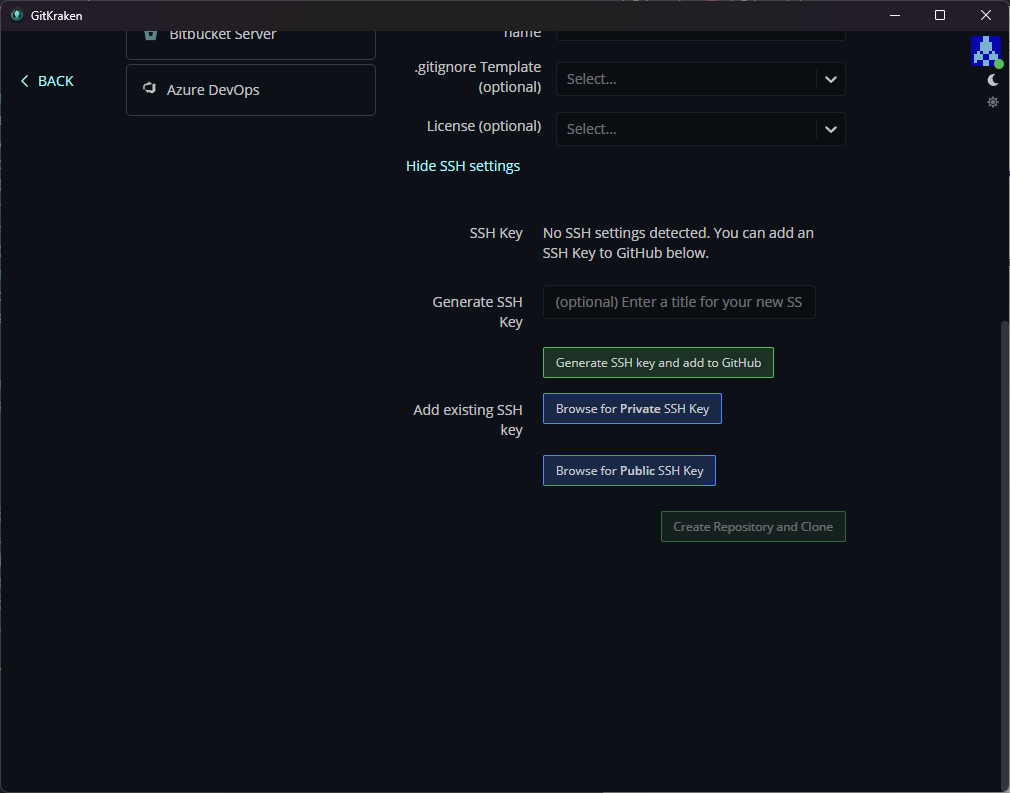
\includegraphics[width=0.8\textwidth]{images/ssh.png}
    \caption{Klonowanie z SSH w GitKraken}
\end{figure}

\newpage
\clearpage

\subsection{Kopia zapasowa}
GitKraken nie posiada opcji do tworzenia kopii zapasowej. Można natomiast użyć do tego celu polecenia archive w wbudowanym terminalu.
\begin{lstlisting}[caption={Kopia zapasowa w terminalu},captionpos=b]
    $ git archive --output=./SiNWO_2.zip --format=zip HEAD ./build
\end{lstlisting}
\begin{figure}[ht]
    \centering
    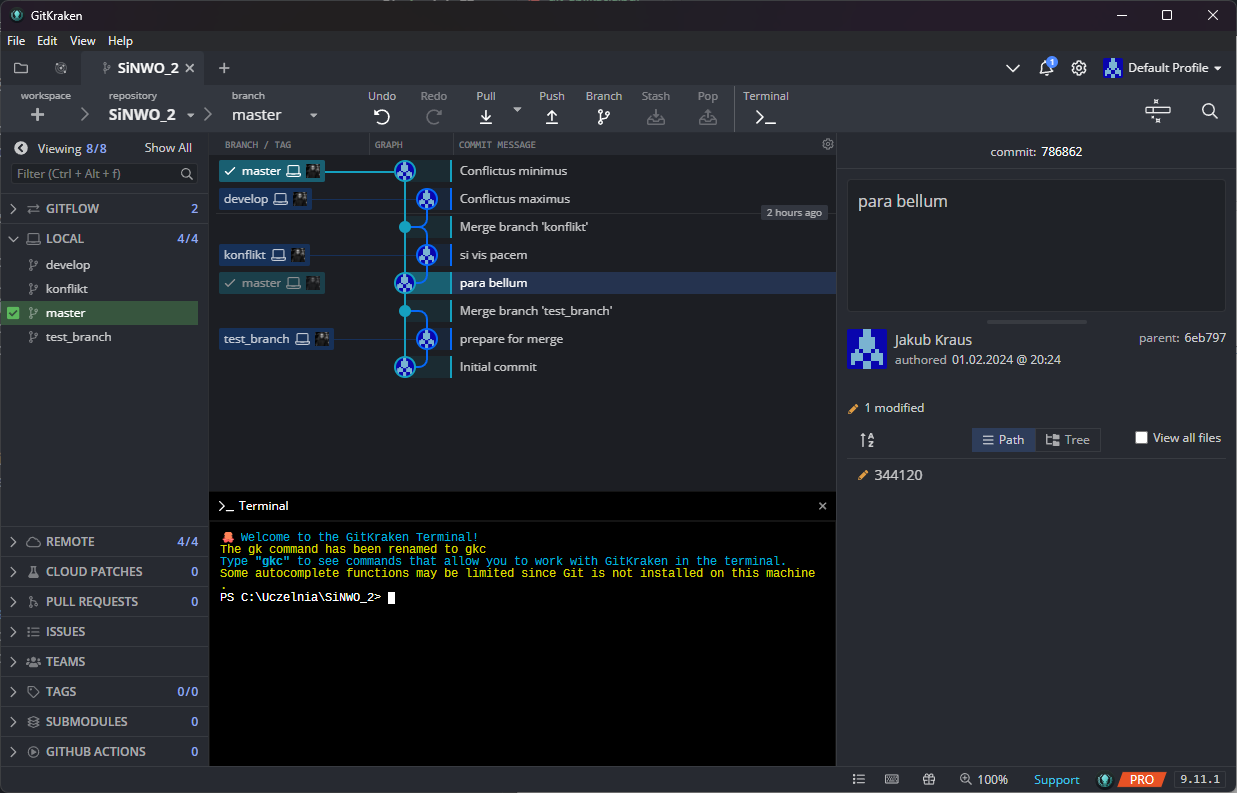
\includegraphics[width=0.8\textwidth]{images/backup.png}
    \caption{Kopia zapasowa w GitKraken}
\end{figure}

\newpage
\clearpage

\subsection{GitFlow}
Gitflow to model rozwoju oprogramowania oparty na systemie kontroli wersji Git. Został stworzony przez Vincenta Driessena i opisany w jego artykule. Model ten ma na celu ułatwienie pracy zespołom programistycznym, zwłaszcza w projektach oprogramowania o większym zakresie.
\subsubsection{Gałąź Master}
Jest to główna gałąź (branch) zawierająca kod produkcyjny. Każda zmiana akceptowana do produkcji jest zintegrowana z tej gałęzi.
\subsubsection{Gałąź Develop}
Gałąź ta jest używana jako gałąź podstawowa dla pracy zespołu. Zawiera najnowsze zmiany i funkcje, które są w trakcie rozwoju.
\subsubsection{Gałąź Feature}
Dla każdej nowej funkcji lub zadania tworzy się oddzielną gałąź. Zmiany te są wprowadzane i testowane na tej gałęzi, a następnie integrowane z gałęzią Develop po zakończeniu prac.
\subsubsection{Gałąź Release}
Przed wypuszczeniem nowej wersji oprogramowania, tworzona jest gałąź Release. Na tej gałęzi dokonuje się ostatnich poprawek, testów i przygotowań do wersji produkcyjnej.
\subsubsection{Gałąź Hotfix}
Jeśli po wypuszczeniu nowej wersji produkcyjnej pojawią się pilne błędy wymagające szybkiej naprawy, tworzona jest gałąź Hotfix. Po naprawieniu błędu, zmiany są integrowane zarówno z gałęzią Master, jak i Develop.

\subsubsection{Schemat prac}

\begin{itemize}
    \item Nowe funkcje i zadania są rozwijane na gałęziach Feature.
    \item Po ukończeniu funkcji, gałąź Feature jest scalana z gałęzią Develop.
    \item Przed wydaniem nowej wersji tworzona jest gałąź Release. Na tej gałęzi dokonywane są ostatnie prace i testy.
    \item Po zakończeniu testów gałąź Release jest scalana z gałęzią Master, a także integrowana z gałęzią Develop, aby uwzględnić ostatnie zmiany.
    \item Na gałęzi Master można utworzyć gałąź Hotfix, aby szybko naprawić błędy na produkcji.
    \item Po naprawie, gałąź Hotfix jest integrowana zarówno z gałęzią Master, jak i Develop.
\end{itemize}

\subsubsection{Podsumowanie}
Model Gitflow pomaga w zarządzaniu procesem rozwoju oprogramowania, zwłaszcza w projektach, które wymagają równoczesnej pracy nad wieloma funkcjami. Dzięki klarownym gałęziom i regułom scalania, ten model przyczynia się do utrzymania porządku w repozytorium, a także umożliwia skuteczne zarządzanie wersjami oprogramowania.

\newpage
\clearpage

\section{Wnioski}
Po przeprowadzeniu działań z wykorzystaniem GitKrakena, można stwierdzić, że narzędzie to dostarcza intuicyjny interfejs graficzny, ułatwiający  pracę z systemem kontroli wersji Git. Funkcje takie jak "Blame", "Checkout", czy "Merge" są łatwo dostępne i wygodne w użyciu, co przyspiesza i ułatwia codzienną pracę programistyczną.

Rozwiązanie konfliktów scalania w GitKraken odbywa się sprawnie dzięki wbudowanemu mergetoolowi, który wspomaga użytkowników podczas rozstrzygania problemów. Jednak warto zauważyć, że umiejętność manualnego rozwiązywania konfliktów poprzez edycję plików jest równie istotna.

Podczas korzystania z GitKrakena, klonowanie repozytorium przy użyciu SSH jest zadaniem prostym do wykonania dzięki intuicyjnemu interfejsowi graficznemu. Działa to efektywnie, szczególnie dla użytkowników, którzy wolą unikać linii poleceń. Niestety tego nie można powiedzieć o tworzeniu kopii zapasowej, które wymaga użycia wbudowanego terminala. W tym przypadku, użytkownicy, którzy nie są zaznajomieni z polecaniami Git w linii poleceń, mogą mieć problemy z wykonaniem tego zadania.

W kontekście preferencji co do narzędzi do kontroli wersji, wybór GitKrakena wynika głównie z jego przyjaznego interfejsu i łatwości obsługi, co przekłada się na szybszą i bardziej efektywną pracę. Jednak dla zaawansowanych użytkowników, znajomość poleceń Git w linii poleceń pozostaje kluczowym elementem, a zrozumienie różnic pomiędzy tymi dwiema formami pracy może być korzystne w zróżnicowanym środowisku programistycznym.

\printbibliography[
    heading=bibintoc,
    title={Bibliografia}
]
\nocite{*}

\end{document}